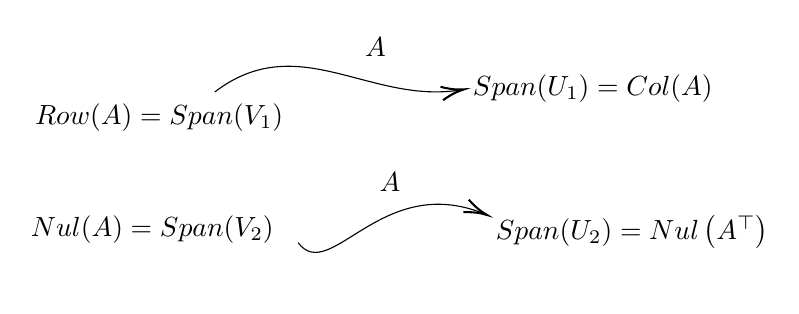
\begin{tikzpicture}[x=0.75pt,y=0.75pt,yscale=-1,xscale=1]
%uncomment if require: \path (0,300); %set diagram left start at 0, and has height of 300


% Text Node
\draw (278,88.4) node [anchor=north west][inner sep=0.75pt]    {$\text{Span}(U_{1}) =\text{Col}(A)$};
% Text Node
\draw (289,156.4) node [anchor=north west][inner sep=0.75pt]    {$\text{Span}(U_{2}) =\text{Nul}\left( A^{\top }\right)$};
% Text Node
\draw (67,102.4) node [anchor=north west][inner sep=0.75pt]    {$\text{Row}(A) =\text{Span}(V_{1})$};
% Text Node
\draw (65,156.4) node [anchor=north west][inner sep=0.75pt]    {$\text{Nul}(A)=\text{Span}(V_{2})$};
% Text Node
\draw (226,70.4) node [anchor=north west][inner sep=0.75pt]    {$A$};
% Text Node
\draw (233,135.4) node [anchor=north west][inner sep=0.75pt]    {$A$};
% Connection
\draw    (195,170.6) .. controls (210.41,191.15) and (235,136.53) .. (284.49,156.63) ;
\draw [shift={(286,157.26)}, rotate = 203.39] [color={rgb, 255:red, 0; green, 0; blue, 0 }  ][line width=0.75]    (10.93,-3.29) .. controls (6.95,-1.4) and (3.31,-0.3) .. (0,0) .. controls (3.31,0.3) and (6.95,1.4) .. (10.93,3.29)   ;
% Connection
\draw    (154.9,98) .. controls (195.13,67.3) and (229.57,104.33) .. (273.66,96.98) ;
\draw [shift={(275,96.74)}, rotate = 169.44] [color={rgb, 255:red, 0; green, 0; blue, 0 }  ][line width=0.75]    (10.93,-3.29) .. controls (6.95,-1.4) and (3.31,-0.3) .. (0,0) .. controls (3.31,0.3) and (6.95,1.4) .. (10.93,3.29)   ;

\end{tikzpicture}